%\documentclass[11pt]{amsproc}
%\documentclass[11pt]{article}
\documentclass[11pt]{article}
%\usepackage{setspace}
%\usepackage{fancyhdr}
\usepackage{fullpage}
\usepackage{graphicx}
\usepackage{amssymb}
%\usepackage{accents}
\usepackage{amsfonts}
\usepackage{amsthm}
\usepackage{amsmath}
\usepackage{eucal}
\usepackage{xypic}
\usepackage{pdfsync}
\usepackage{hyperref}
\usepackage{enumerate}



%%\setrightmargin{1in}
%\setallmargins{1in}

% Titlerule is a FAT ruler
\newcommand{\titlerule}{\rule{\linewidth}{1.5mm}}
% For comments in the draft - work in progress
\newcommand{\betainsert}[2]{\fbox{#1}\marginnote{\textsf{#2}}}

% Notes in the margin are nicer this way. HaHa
\newcommand{\marginnote}[1]{\marginpar{\scriptsize\raggedright #1}}



\def\bd{\partial}
\def\ra{\rightarrow}
\def\lra{\longrightarrow}
\def\Z{{\mathbb Z}}
\def\N{{\mathbb N}}
\def\R{{\mathbb R}}
\def\Q{{\mathbb Q}}
\def\C{{\mathbb C}}
\def\P{{\mathbb P}}
\def\K{{\mathbb K}}
\def\w{\mathcal{W}(E)}
\def\A{\mathcal{A}}
\def\B{\mathcal{B}}
\def\M{\mathcal{M}}
\def\N{\mathcal{N}}
\def\p{\partial}

\newcommand*{\longhookrightarrow}{\ensuremath{\lhook\joinrel\relbar\joinrel\rightarrow}}

\newtheorem{lem}{Lemma}
\newtheorem{prop}{Proposition}
\newtheorem{thm}{Theorem}
\newtheorem{cor}{Corollary}
\newtheorem{conj}{Conjecture}
\newtheorem{defn}{Definition}
\newtheorem{claim}{Claim}
\newtheorem{ques}{Question}
\newtheorem{rem}{Remark}

\theoremstyle{remark}
\newtheorem*{prob}{Problem}
\newtheorem{ex}{Example}
\def\T{\mathbb{T}}

\begin{document}
\begin{center}
    \begin{Large} {\bf Math 540 Homework 3}\\
    \end{Large}
    Haosen Wu  / Friday, Sept. 14, 2018
\end{center}
%\vspace{10mm}
\subsection*{1 Group Law}
\begin{itemize}
    \item a. $(AB)C=
    (b^2a^{-1}b^{-3}ab^{-1}ab^{-2}b^2a^{-1}ba^{-1}bab^2)b^{-2}a^{-1}b^2a^3b=
    (b^2a^{-1}b^{-2}ab^2)b^{-2}a^{-1}b^2a^3b=
    b^2a^2b=
    b^2a^2b=
    b^2a^{-1}b^{-3}ab^{-1}ab^{-2}(b^2a^{-1}ba^{-1}b^3a^3b)=
    b^2a^{-1}b^{-3}ab^{-1}ab^{-2}(b^2a^{-1}ba^{-1}bab^2b^{-2}a^{-1}b^2a^3b)=
    A(BC)$ very beautiful, my eyes report.
    \item b. $(AB)D=
    (b^2a^{-1}b^{-3}ab^{-1}ab^{-2}b^2a^{-1}ba^{-1}bab^2)b^{-2}a^{-1}b^2ab^{-2}a^3=
    (b^2a^{-1}b^{-2}ab^2)b^{-2}a^{-1}b^2ab^{-2}a^3=
    a^3=
    a^3=
    (b^2a^{-1}b^{-3}ab^{-1}ab^{-2}b^2a^{-1}ba^{-1}b^3ab^{-2})a^3=
    b^2a^{-1}b^{-3}ab^{-1}ab^{-2}(b^2a^{-1}ba^{-1}b^3ab^{-2}a^3)=
    b^2a^{-1}b^{-3}ab^{-1}ab^{-2}(b^2a^{-1}ba^{-1}bab^2b^{-2}a^{-1}b^2ab^{-2}a^3)=
    A(BD)$ 
    \item c. My eyes hate LaTeX now.
\end{itemize}

\subsection*{2 Group infini }
\begin{itemize}
    \item a. $G=<a,b;a^2b^{-3}=1>$, the permutation group is $S_3$.
    Let $S=\textrm{\{}a,b\textrm{\}}$, We consider a map $\varphi$ defined by $\varphi: S \rightarrow S_3$ with $\varphi(e)=e,\varphi(a)=(1\textrm{ }2)$ and $\varphi: S \rightarrow S_3$ with $\varphi(e)=e,\varphi(b)=(1\textrm{ }2 \textrm{ }3) ,\varphi(b^2)=(1\textrm{ }3 \textrm{ }2)$. Therefore from the universal property of free group we have the following diagram commute
    \[
    \xymatrix{
    S \ar[r]^{i}\ar[dr]^{\varphi} & F(S) \ar[d]^{f}&  \\
    & S_3 &
    }
    \]
     Then we have the desired $f$ from the universal property, which is also asserted unique, in particular, $Ker(f)$ contains $a^2b^{-3}$ since $f(a^2b^{-3})=f(a^2)f(b^{-3})=f^2(a)f^{-3}(b)=1\cdot 1=1$. Then we can descend $f$ to $\tilde{f}:G=<a,b;a^2b^{-3}=1> \rightarrow H$, the $\tilde{f}$ is the desired morphism, the following diagram commute.
    \[
    \xymatrix{
    S \ar[r]^{i}\ar[dr]^{\varphi} & F(S) \ar[d]^{f}& \ar[r]_{p}\ar[dl]_{\tilde{f}} G\\
    & S_3 &
    }
    \]
     
     Also $\tilde{f}$ maps $a,b$ to desired $\tau,\rho$: $\tilde{f}(a)=\restr{f}_{G}(a)=\restr{\varphi}_{S}(a)=\varphi(a)=(1\textrm{ }2) $ and $\restr{f}_{G}(b)=\varphi'(b)=\restr{\varphi}_{S}(b)=(1\textrm{ }3 \textrm{ }2)$. 
     
    We start showing $G$ is not abelian by assuming $G$ is. Then we shall have $f(ab)=f(ba)$ since $ab=ba$, however $S_3 $ is not an abelian group, therefore $f(a)f(b)=(1\textrm{ }3)\neq(3\textrm{ }2)=f(b)f(a)$ so we arrive a contradiction.
    
    \item b. We find an explicit map $\phi:G\rightarrow \Z$: $\phi(a)\rightarrow 3$,  $\phi(b)\rightarrow 2$ and $\phi(a^mb^n)\rightarrow m\phi(a)+n\phi(b) $. We can verify $\phi$ is a homomorphism: $\phi(a^mb^n)=m\phi(a)+n\phi(b)=3m+2n=\phi(a^m)\phi(b^n)$,
    in particular, plug $m=2,n=-3$ we obtain $0$. This homomorphism is also an epimorphism since $\phi((ab^{-1})^n)=n\phi((ab^{-1})^n)=n(3-2)=n$, therefore $|G|>|Z|=\infty$.
    
\end{itemize}

\newpage
\subsection*{3 Group }
\begin{itemize}
    \item $\pi_2$ gives second-homotopy class in $X$; 
    Precisely, let $h_1,h_2$ be paths $h_1,h_2:[0,1]\rightarrow X$, and by homotopy connecting $x_0$ to $h_i$ then $x_0$, in forms of 
    \[
    H_i(s,t):= \begin{cases} x_0(1-2t)+2th_i(s) & \text{when } 0\leq t \leq 1/2 \\ x_0(2t-1)+(2-2t)h_i(s) & \text{otherwise.} \end{cases}
    \]
    where $H_i: [0,1]\times[0,1] \rightarrow X$, such modulo homotopy of the homotopy, defined as equivalence relation $\tilde{H}(-,0)=H_i \sim H_j=\tilde{H}(-,1) $, where $ \tilde{H}: [0,1]\times[0,1]\times[0,1]\rightarrow X$. 
    Thus indeed $\pi_2$ refers to higher (second) homotopy class.  
    
    The reason of $H_i$ be homotopy is by pasting lemma: when $t=1/2$, first part gives $H(-,1/2)=h_i(s)$ and second part gives $H(-,1/2)=h_i(s)$ as well. The reason of $\tilde{H}$ be homotopy is by proof of (2) in Homework $1$, since (first) homotopy $H_i$ is regarded as path in $\Omega_{x_0}X$, then $\tilde{H}$ is indeed the homotopy of paths in $\Omega_{x_0}X$  by construction. //
    
    That is saying, we inherit group law since we define $\pi_2$ as $\pi_1(\textrm{Top Space})$, and the order of composing homotopies (as path in $\Omega_{x_0}X$), from different equivalence class, does not matter up to homotopy, for $\beta \in [\beta]$ and $\alpha \in [\alpha]$, $\beta \ast \alpha \simeq \alpha \ast \beta \Leftrightarrow H_\beta \ast H_\alpha \simeq H_\alpha \ast H_\beta $.
    
    \item Geometrically speaking we can "rotate" $\alpha,\beta$ to reach the homotopy between $\beta \ast \alpha$ and $\alpha \ast \beta$. Practically to show $\pi_2(S^1;x_0) $ is abelian is to show for all $[\alpha],[\beta] \in \pi_2(S^1;x_0)$ we have $[\alpha]\ast[\beta] = [\beta]\ast[\alpha]$, which is equivalent to for representative elements $\alpha \in[\alpha],[\beta] \in[\beta]$, $\alpha \ast \beta \simeq \beta \ast \alpha$. Since we mentioned that path in $\Omega_{x_0}X$ is path-homotopy in $X$, we now give $\alpha(t)=H_\alpha(-,t)$, as well as $\alpha \ast \beta= H_\alpha \ast H_\beta(= H_{\alpha \ast \beta})$ [The concatenation is by pasting and makes sense since all $H_i$ have the same start/end path(point) $c_{x_0}$, by defined.]
    
    Now we notice that  $\pi_2(S^1;x_0)=\pi_1(\Omega_{x_0}X;c_{x_0})$ then by the proven, we consider the homotopy of the homotopy squares: contracting domain of $\alpha,\beta$, then we can "rotate" and deflating $\alpha,\beta$ back, explicitly  
    \[
    \tilde{H}(s,t,t'):= \begin{cases} 
    \begin{cases}
     H_\alpha(2s,2(t-3t'/2)) & \text{} 0\leq s \leq 1/2, 0\leq t \leq 3t'/2,  0 \leq t' \leq 1/3 \\ 
     H_\beta(2s-1,1-2(t-3t'/2)) & \text{} \\
     x_0 & \text{otherwise} 
     
    \end{cases} \\
    
    \begin{cases}
     H_\alpha(2(s-3(t'-1/3)/2),t) & \text{} 3(t'-1/3)/2\leq s \leq 1/2+3(t'-1/3)/2, \\
     H_\beta(2(s-3(t'-1/3)/2)-1,t) & \text{} 0\leq t \leq 1, 0 \leq t' \leq 1/3 \\
     x_0 & \text{otherwise} 
     
    \end{cases} \\

    \begin{cases}
     H_\alpha(2(s-1/2),1-2(t+3t'/2-3/2)) & \text{} 1/2\leq s \leq 1, -3/2t'+3/2\leq t \leq 1,\\ 
     H_\beta(2(s-1/2)-1,2(t+3t'/2-3/2)) & \text{}  2/3 \leq t' \leq 1 \\
     x_0 & \text{otherwise} 
     
    \end{cases} \\
    \end{cases}
    \]
    
    We thus have $\tilde{H}(s,t,0)=H_{\alpha * \beta}$ and $\tilde{H}(s,t,1)=H_{\beta * \alpha}$, that is, $\beta \ast \alpha \simeq \alpha \ast \beta $.
    This is really a homotopy since 1) it is a composition of $H_i(-)$ and $linear \textrm{ }function(s,t,t')$, which are both continuous functions and 2) on the gluing part pasting lemma applies. (#)
    
    A 3D diagram is belowm (Figure 3b).
    \begin{figure}[h!]
    \centering
    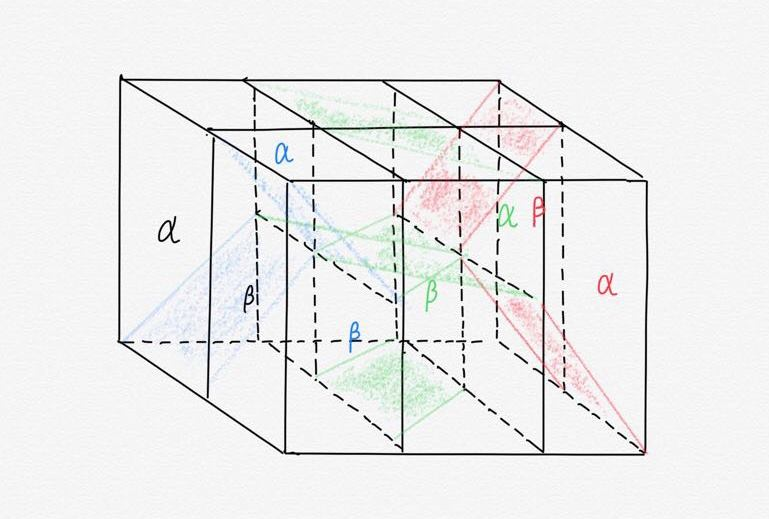
\includegraphics[scale=0.33]{IMG_0273}
    \caption{3b}
    \end{figure}
    
    \item Let us call previous $\tilde{H}$ as $H^2$, denote for $2$-th homotopy; then we have following $H^n$, denote for $n$-th homotopy. Define $\pi_n$ as stated.
    
    $\pi_n$ comprises of $1$-dimension higher homotopy class in $\pi_{n-1}$, given by homotopy of the homotopy $\dots$ of the homotopy (for $n-1$ times)
    $H^{n-1}(s,t_0,...,t_{n-2})$ as $H^{n-1}: [0,1]\times[0,1]\times\dots\times [0,1] \rightarrow X$, then
    modulo homotopy of the homotopy $\dots$ of the homotopy (for $n$ times), which is $H^n:   [0,1]\times[0,1]\times\dots\times [0,1] \rightarrow X$.
    
    
    \item Similar to the abelian property of $\pi_2$, we have higher $\pi_n$ group with the commutativity for path elements for $p_i,p_j \in \Omega^{n-1}_{x_0}X$, $[p_i]\ast[p_j]=[p_j]\ast[p_i]$, due to our concatenation on the point $c_{x_0}$. We thus can always by "rotation" argument in (b), construct $\tilde{H}(s,t_1,...,t_{n-1}): [0,1]^ \rightarrow X$ with descending first $[0,1]^{n-1}$ dimensions to $[0,1]\times[0,1]$ and thus fit $\tilde{H}$ in Figure  3b, then we obtain required homotopy $\tilde{H}(s,t_1,...,t_{n-1})$ (again $\tilde{H}$ is a homotopy for same reason # in 3b.) such that when taking representatives $p_i,p_j\textrm{from}[p_i],[p_j]$, $\tilde{H}(s,t_1,...,0)=H_i(s,t_1,...,t_{n-2})\ast H_j(s,t_1,...,t_{n-2})=p_i\ast p_j \simeq p_j\ast p_i=H_i(s,t_1,...,t_{n-2})\ast H_i(s,t_1,...,t_{n-2})=\tilde{H}(s,t_1,...,1)$ , this finishes proof for $n$-th group case.
    
    
    \subsection*{Fundamental Group I}
  Recall SvK Theorem I. We have deformation retract diagrams as Figure $1$ for $\R^1,\R^2,\R^n$ cases, labeled as $X_1,X_2,X_n$. $\R^1$ case is like line with $p$-divides,$\R^2$ case is like $B^2$ with $p$-holes, $R^n$ deserves an explanation: $R^n$ is open and closed???. Thus correspondingly, for $X_1$ since the only path-connected space is line, $\pi_1(X_1)=1$;  for $X_2$ by diagram we proceed induction on $p$: for solely $1$ p we have $\pi_1(X_2_1)=\pi_1(X_2_1)=\Z$ and $\pi_1(X_2_1\cap X_2_2)=1$ then we see all maps $i:\pi_1(X_2_1\cap X_2_2) \rightarrow \pi_1(X_2_i)$ are trivial. The amalgamated product degenerates to free product. Thus $\pi_1(X_2_1\cup X_2_2)=\Z*\Z$. for $n$ p we have assume $\pi_1(\bigcup X_2_i)=*_n\Z$, we also recognize  $\pi_1((\bigcup_n X_2_i)\cap X_2_{n+1})=1$, and amalgamated product degenerates again thus $\pi_1((\bigcup_{n+1} X_2_i)=*_{n+1}\Z$; for $X_n$ since the space is simply and path connected we get $\pi_(X_2)=1$ immediately. 
    
\end{itemize}

\end{document}